% Created 2024-10-16 śro 21:35
% Intended LaTeX compiler: pdflatex
\documentclass[../main.tex]{subfiles}

% \usepackage[a4paper, margin=3cm]{geometry}
% \usepackage{amssymb} // not working

\usepackage[T1]{fontenc}
\usepackage[utf8]{inputenc}
\usepackage{graphicx}
\usepackage{longtable}
\usepackage{wrapfig}
\usepackage{rotating}
\usepackage[normalem]{ulem}
\usepackage{amsmath}
\usepackage{capt-of}
\usepackage{hyperref}
\usepackage{siunitx}
\usepackage{float}
\usepackage[polish]{babel}

\graphicspath{{../}}
\author{Wojciech Paderewski}
\date{\today}
\title{Koncepcja układu}
\hypersetup{
 pdfauthor={Wojciech Paderewski},
 pdftitle={Koncepcja układu},
 pdfkeywords={},
 pdfsubject={},
 pdflang={Polish}}

\begin{document}
Bazując na informacjach z podrozdziału \ref{sec:srodowisko_programistyczne}, wybrano środowisko programistyczne PlatformIO, które jest wtyczką do Visual Studio Code. 
Zaletą tego rozwiązania nad Arduino IDE są podpowiedzi składniowe, co znacząco przyspiesza pisanie kodu.
PlatformIO pozwala również na łatwe zarządzanie bibliotekami, komunikację z użyciem portu szeregowego oraz możliwość debugowania kodu.

Określono wymagania, które musi spełniać oprogramowanie:
\begin{itemize}
  \item Obsługa rejestrów przesuwnych w celu wyświetlenia cyfr na lampach Nixie.
  \item Połączenie z siecią Wi-Fi.
  \item Pobranie czasu z serwera czasu.
  \item Obsługa enkodera obrotowego.
  \item Komunikacja z potencjometrem cyfrowym w celu zmiany jasności wyświetlacza.
  \item Odczyt obecnego napięcia na przetwornicy wysokiego napięcia.
  \item Odtwarzanie dźwięku za pomocą głośnika piezoelektrycznego.
  \item Komunikacja z serwerem Home Assistant przez protokół MQTT.
\end{itemize}

W celu zrealizowania powyższych wymagań program został podzielony na moduły, które są odpowiedzialne za poszczególne funkcjonalności.
Taki podział pozwolił też na testowanie poszczególnych funkcjonalności niezależnie od siebie i połączenie ich w pliku \texttt{main.cpp}.

\subsection{Sterowanie lampami Nixie}
W celu wyświetlenia cyfr na lampach Nixie moduł podzielono na 4 warstwy abstrakcji:
\begin{itemize}
  \item Klasę samego rejestru przesuwnego, który pozwala na wysłanie 64 bitów danych do rejestru przesuwnego.
  \item Klasę wyświetlacza, który pozwala na wyświetlenie cyfry na konkretnym wyświetlaczu Nixie.
  \item Zdefiniowane struktury łączące cyfrę z konkretnym bitem w rejestrze przesuwnym.
  \item Klasę do animacji wyświetlacza.
\end{itemize}

Wysyłanie danych do rejestru odbywa się za pomocą funkcji \texttt{send} w klasie \texttt{ShiftRegisterExpander}.

\begin{verbatim}
    void send() {
        for (size_t i = 0; i < this->outputCount; i++) {
            digitalWrite(regClkPin, HIGH);
            if (this->outputs[this->outputCount - i - 1]) {
                digitalWrite(regDataPin, HIGH);
            } else {
                digitalWrite(regDataPin, LOW);
            }
            digitalWrite(regClkPin, LOW);
            esp_rom_delay_us(1);
        }

        // latch toggle
        digitalWrite(regLePin, HIGH);
        esp_rom_delay_us(1);
        digitalWrite(regLePin, LOW);
        esp_rom_delay_us(1);
    }
\end{verbatim}


Animacja cyfr polega na zapaleniu każdej z cyfr pomiędzy 0 a obecnie wyświetlaną cyfrą, w momencie zmiany danej cyfry na 0.
Funkcjonalność ta jest zrealizowana w klasie \texttt{AnimationDriver} w metodzie \texttt{update}.

\begin{verbatim}
    void update() {
        if (this->desiredDigit == this->currentDigit) {
            return;
        }

        if (!this->animating) {
            this->nixie.setDigit(this->desiredDigit);
            this->currentDigit = this->desiredDigit;
            return;
        }

        uint8_t animationStep = (millis() - this->startTime) / 50;

        if (animationStep > 9) {
            this->animating = false;
            this->currentDigit = this->desiredDigit;
            this->nixie.setDigit(this->desiredDigit);
            return;
        }

        uint8_t animatedDigit = 9 - animationStep;
        if (animatedDigit < this->currentDigit) {
            this->nixie.setDigit(animatedDigit);
            this->currentDigit = animatedDigit;
            return;
        }
    }
\end{verbatim}

\subsection{Połączenie z siecią Wi-Fi}
W celu połączenia z siecią Wi-Fi, wykorzystano bibliotekę \texttt{WiFi.h} dostępną w środowisku PlatformIO. Dodatkowo by nie trzymać hasła do sieci na repozytorium, ze wzgledow bezpieczeństwa,
stworzono oddzielny plik \texttt{secret.hpp}, w którym przechowywane są dane do połączenia z siecią. Do incjalizacji połączenia z siecią służy funkcja \texttt{WIFI\_Init}.

\begin{verbatim}
    void WIFI_Init() {
        Serial.println("[wifi] Starting WiFi");
    
        WiFi.mode(WIFI_STA);
        WiFi.begin(ssid, password);
    
        Serial.print("[wifi] Connecting to network ssid: ");
        Serial.print(ssid);
        Serial.print(" password: ");
        Serial.println(password);
    
        while (WiFi.status() != WL_CONNECTED) {
            Serial.println("[wifi] Waiting for connection...");
            delay(1000);
        }
    
        Serial.print("[wifi] Connected to network with IP: ");
        Serial.println(WiFi.localIP());
    }
\end{verbatim}

\subsection{Pobranie czasu z serwera czasu}
W celu pobrania czasu z serwera czasu, wykorzystano bibliotekę \texttt{NTPClient.h} oraz \texttt{WiFiUdp.h} dostępne w środowisku PlatformIO.
Do komunikacji z serwerem czasu służą następujące funkcje:

\begin{verbatim}
    void NTP_Init() {
        timeClient.begin();
        timeClient.setTimeOffset(3600 * 1);
    }
    
    void NTP_Update() {
        timeClient.update();
    }
    
    uint32_t NTP_GetTime() {
        return timeClient.getEpochTime();
    }
    
    uint8_t NTP_GetHour() {
        return timeClient.getHours();
    }
    
    uint8_t NTP_GetMinute() {
        return timeClient.getMinutes();
    }
    
    uint8_t NTP_GetSecond() {
        return timeClient.getSeconds();
    }
    
\end{verbatim}

\subsection{Obsługa enkodera rotacyjnego}
Moduł enkodera rotacyjnego został zaimplementowany w klasie \texttt{Encoder}. Klasa ta zlicza impulsy z enkodera oraz zapisuje kierunek obrotu enkodera.
Klasa ta bazuje na mechanizmie callbacków, które są wywoływane w momencie zmiany stanu pinów enkodera. Inne moduły mogą reagować na zmianę stanu enkodera poprzez zarejestrowanie callbacka.
Dostępne są następujące callbacki:

\begin{verbatim}
    std::function<void()> rightCallback;
    std::function<void()> leftCallback;
    std::function<void()> switchPressCallback;
    std::function<void()> switchReleaseCallback;
\end{verbatim}

\subsection{Reguluja i odczyt napięcia} 
Komunikacja z potencjometrem cyfrowym odbywa się za pomocą interfejsu I2C.
 W celu komunikacji z potencjometrem, wykorzystano bibliotekę \texttt{Wire.h}. Wykorzystany potencjometr jest 128-stopniowy, z informacji z 
 karty katalogowej \cite{st:potencjometr} wynika, że ramka danych ma się składać z adresu urządzenia(podanego w dokumentacji) oraz wartości korku w zakresie od 0 do 127.
 Na postawicie tych informacji w klasie \texttt{HVConverter} zaimplementowano funkcje do ustawienia wartości potencjometru \texttt{sendPotSteps} oraz funkcję 
 do przeliczania zadanego napięcia na wartość potencjometru \texttt{voltageToSteps}.

\begin{verbatim}
    #define MAX_VOLTAGE 210
    #define MIN_VOLTAGE 134
    #define POT_STEPS 127
    #define POT_ADDR 0x2F
    #define OFFSET 4

    void sendPotSteps(uint8_t steps) {
        Wire.beginTransmission(POT_ADDR);
        Wire.write(steps);
        Wire.endTransmission();
    }
    
    int voltageToSteps(uint8_t v) {
        return (v + OFFSET - MIN_VOLTAGE) * POT_STEPS / (MAX_VOLTAGE - MIN_VOLTAGE);
    }

\end{verbatim}

Klasa \texttt{HVConverter} ma również zaimplementowaną funkcję do odczytu napięcia na przetwornicy, która bazuje na pomiarze napięcia na dzielniku napięcia za pomocą 
wbudowanego 12 bitowego przetwornika ADC. Funkcja ta zwraca wartość napięcia w mV, co następnie jest przeliczane na wartość napięcia na przetwornicy, za pomocą 
funkcji liniowej.

\begin{verbatim}
    #define R1 10 000
    #define R2 1 000 000

    uint16_t readVoltage() {
        uint16_t rawValueMilliVolts = analogReadMilliVolts(voltageMeasurePin);
        uint16_t rawVoltageInVolts = rawValueMilliVolts / 1000;
        return rawVoltageInVolts * (R1 + R2) / R2;
    }
\end{verbatim}

\subsection{Odtwarzanie dźwięku}
Do odtwarzania dźwięku wykorzystano funkcje \texttt{tone} oraz \texttt{noTone} dostępne w środowisku, do generowania sygnału o zadanej częstotliwości.
Same melodie są zdefiniowane w pliku \texttt{melody.hpp}, a poszczególne tony w pliku \texttt{tones.hpp}. Same melodie są zdefiniowane jako tablice tonów oraz tablice długości tonów.
W celu lepszej czytelności kodu, stworzono strukturę \texttt{Melody}, która przechowuje tablice tonów oraz długości tonów.

\begin{verbatim}
    struct Melody {
        String name;
        std::vector<int> tones;
        std::vector<int> noteDurations;
    };
    
    // Przykładowa melodia
    Melody happyBirthdayMelody = {
        .name = "Happy Birthday",
        .tones = {
            NOTE_C4, NOTE_C4, NOTE_D4, NOTE_C4, NOTE_F4, NOTE_E4,
            NOTE_C4, NOTE_C4, NOTE_D4, NOTE_C4, NOTE_G4, NOTE_F4,
            NOTE_C4, NOTE_C4, NOTE_C5, NOTE_A4, NOTE_F4, NOTE_E4, NOTE_D4,
            NOTE_AS4, NOTE_AS4, NOTE_A4, NOTE_F4, NOTE_G4, NOTE_F4},
        .noteDurations = {400, 400, 400, 400, 400, 200, 400, 400, 400, 400, 400, 200, 400, 400, 400, 400, 400, 400, 200, 400, 400, 400, 400, 400, 200}};
\end{verbatim}

Samo odtwarzanie dzwieku dzieje się w klasie \texttt{Buzzer}, pozwala ona na ustawienie zadanej melodii, odtworzenie melodii oraz zatrzymanie odtwarzania.
Samo odtwarzanie musi być asynchroniczne, aby nie blokować innych funkcjonalności. 
W tym celu napisano funkcję update, która jest wywoływana w pętli głównej programu.

\begin{verbatim}
    void update() {
        if (!isPlaying) {
            return;
        }
        unsigned long currentTime = millis();
        int adjustedNoteDuration = melody.noteDurations[currentNote];
        if (currentTime - lastNoteTime >= adjustedNoteDuration * 1.30) {
            noTone(buzzerPin);
            currentNote++;
            if (currentNote >= melody.tones.size()) {
                stop();
                return;
            }
            lastNoteTime = currentTime;
        }
        if (melody.tones[currentNote] != 0 &&
            currentTime - lastNoteTime < adjustedNoteDuration) {
            tone(buzzerPin, melody.tones[currentNote]);
        }
    }
\end{verbatim}

\subsection{Komunikacja z serwerem Home Assistant}
Komunikacja z serwerem Home Assistant odbywa się za pomocą protokołu MQTT. W celu komunikacji z serwerem Home Assistant, wykorzystano bibliotekę \texttt{PubSubClient.h}.
Realizację komunikacji z serwerem Home Assistant zaimplementowano w klasie \texttt{MQTT}. Klasa ta pozwala na incjalizacji połączenia z serwerem, 
publikowanie wiadomości oraz obsługę callbacków z serwera. Informacje potrzebne do połączenia z serwerem są przechowywane w pliku \texttt{secret.hpp}.

W tej klasie również przechowywane są dane żądanego stanu przez serwer, który jest urządzeniem nadrzędnym. Są to następujące dane:
\begin{itemize}
  \item \texttt{alarmDesiredHour} - żądana godzina alarmu.
  \item \texttt{alarmDesiredMinute} - żądana minuta alarmu.
  \item \texttt{isAlarmEnabled} - czy alarm jest aktywny.
  \item \texttt{desiredBrightness} - żądana jasność wyświetlacza.
  \item \texttt{desiredMelody} - żądana melodia.
\end{itemize}

Dodawano również oddzielny topic który informuje zegarek że alarm został wyłączony, tak samo zegarek publikuje informacje do serwera o stanie alarmu.
Na podstawie tych zmiennych będą wykonywane działania w pętli głównej programu.

\subsection{Główna logika programu}
Główna logika programu znajduje się w pliku \texttt{main.cpp}. Następuje tu incjalizacji wszystkich obiektów oraz definicja wszystkich pinów i przekazanie ich do obiektów odpowiednich klas.
W funkcji \texttt{setup} inicjalizowane są moduły oraz funkcje co muszą być wykonane tylko raz.
Następnie w pętli głównej programu wywoływane są funkcje update z poszczególnych klas, które są odpowiedzialne za obsługę poszczególnych funkcjonalności.
Schemat działania programu przedstawiony jest na rysunku \ref{fig:schemat_dzialania}. Na schemacie \ref{fig:struktura_programu} przedstawiona jest struktura programu oraz
relacje pomiędzy poszczególnymi modułami.

\begin{figure}[H]
    \centering
    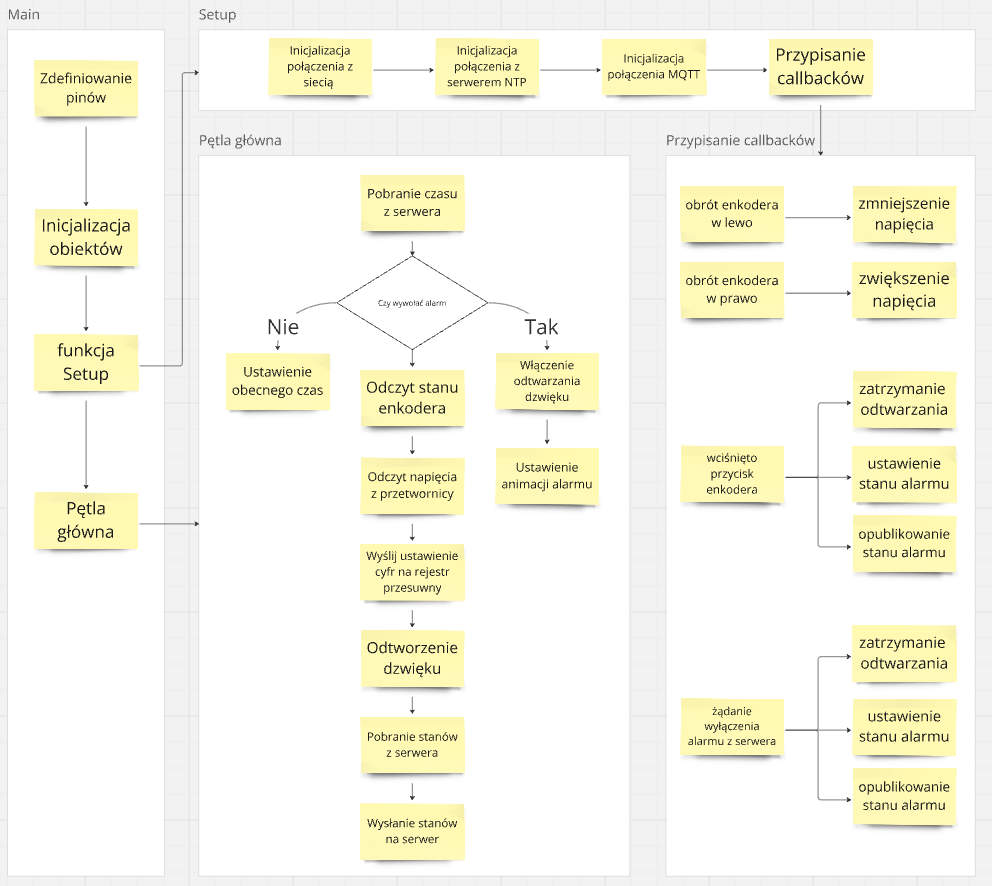
\includegraphics[width=1\textwidth]{program.png}
    \caption{Schemat działania programu}
    \label{fig:schemat_dzialania}
\end{figure}

\begin{figure}[H]
    \centering
    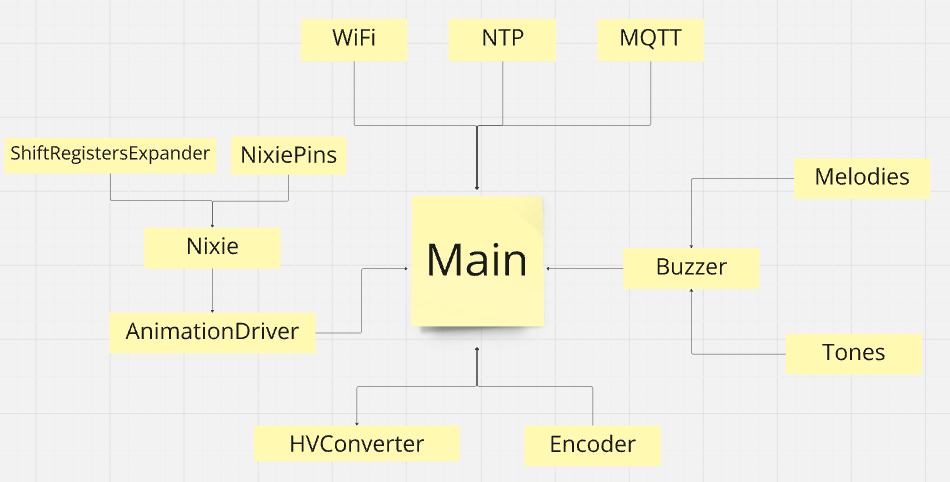
\includegraphics[width=1\textwidth]{Struktura.png}
    \caption{Struktura programu}
    \label{fig:struktura_programu}
\end{figure}

\subsection{Interfejs użytkownika}
Jako interfejs użytkownika służy widget dodany w aplikacji Home Assistant. Środowisko Home Assistant pozwala na tworzenie własnych widgetów,
które są wyświetlane na pulpicie głównym. Widget ten pozwala na ustawienie godziny alarmu na wybrane dni oraz włączenie lub wyłączenie funkcji alarmu.
Widok interfejsu użytkownika przedstawiony jest na rysunku \ref{fig:widget}. Pozostałe funkcje takie jak zmiana jasności wyświetlacza i wyłączanie
alarmu są dostępne wyłącznie na zegarku. W przyszłości planowane jest dodanie dodatkowych funkcji takich jak zmiana melodi alarmu oraz obsługa
paska LED. 

\begin{figure}[H]
    \centering
    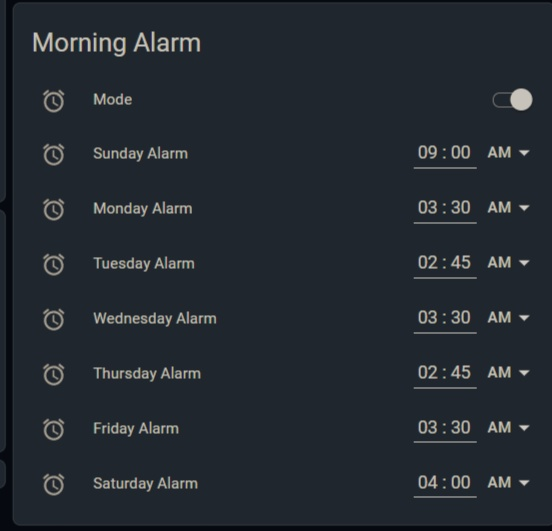
\includegraphics[width=0.7\textwidth]{UI.jpeg}
    \caption{Widget w aplikacji Home Assistant}
    \label{fig:widget}
\end{figure}

\end{document} 